
\documentclass{llncs}

%\documentclass[
%10pt,
%parskip, % Uncomment to add space between paragraphs
%headsepline, % Uncomment to get a line under the header
%twocolumn
%]{article} % The class file specifying the document structure

% \usepackage{pdfcomment}
\usepackage{palatino}
\usepackage[utf8]{inputenc} % Required for inputting international characters
\usepackage[T1]{fontenc} % Output font encoding for international characters
% \usepackage[margin=2.5cm]{geometry}
\usepackage{changepage}
\usepackage{graphicx}

% \geometry{
% 	paper=a4paper, % Change to letterpaper for US letter
% 	inner=2.5cm, % Inner margin
% 	outer=3.8cm, % Outer margin
% 	bindingoffset=2cm, % Binding offset
% 	top=1.5cm, % Top margin
% 	bottom=1.5cm, % Bottom margin
% 	%showframe,% show how the type block is set on the page
% }


\title{Inference of Socioeconomic Status}

\author{
	Martín Fixman\inst{1}
\and
	Esteban Feuerstein\inst{1}
\and 
    Jorge Brea\inst{2}
\and
	Carlos Sarraute\inst{2}
}

\institute{
	Universidad de Buenos Aires, Argentina
\and
    Grandata Labs
}
% \date{}

\begin{document}

\maketitle

\begin{abstract}

La explosión del uso del celular en las comunicaciones en los últimos años se produjo en un momento donde el poder de procesamiento de datos estaba aumentando de manera contundente. Gracias a estos dos cambios a nivel mundial, podemos usar las comunicaciones como una manera de inferir datos sobre los usuarios.

Modelar los datos de las personas dentro de lo que llamamos \textbf{Grafo de Comunicaciones} es crucial para lograr un entendimiento sobre la información demográfica de la población. Nosotros proponemos usar datos provenientes de diferentes fuentes para aproximar el nivel socioeconómico de cada persona en el grafo.

\end{abstract}

\section{Introduction}

% \pdfcomment{Acá van temas sobre papers referenciados, y un resumen de algunas cosas}

\subsection{Data source}

Los datos usados por este estudio consisten de \textbf{Call Detail Records}, o CDRs, sobre llamados y mensajes de texto provenientes de la red de una compañía telefónica Mexicana, en un periodo de \( M \) meses (\( M = 3 \)), denotado por \( L \). Cada CDR contiene los números de teléfonos anonimizados de los dos participantes de la comunicación \(\left<o, d\right>\), el tiempo del llamado \(t\), y, en el caso de los CDRs de llamados su duración \(s\). Un subconjunto de estos llamados también contienen la latitud y la longitud de la antena usada para la llamada, \(\left<y, x\right>\).

\( L \) contiene llamadas y mensajes cuyo origen o destino son los usuarios de la telco, pero no incluye comunicaciones entre la gran cantidad de usuarios que no son parte de esta. Definiendo \( N \) como los usuarios de la telco y \( L_N \) como las llamadas donde \( o \in N \wedge d \in N \), podemos crear un grafo de comunicaciones \( G_N \) que contenga todas las llamadas de cada uno de sus usuarios.

Además se usa información sobre depósitos, extracciones, y transacciones hechas desde bancarias de uno de los bancos más grandes de México, algunas de las cuales incluyen el número de teléfono anonimizado de la misma manera que en los CDRs, por lo cual se puede correlacionar con estos. Usamos los datos durante el mismo periodo de \( M \) meses, denotado por \( B \), los cuales incluyen, por cada usuario hasta 4 teléfonos \( t_0 \cdots t_3 \), e información del monto de sus transacciones \( s_0 \cdots s_n \).

Al igual que en el dataset anterior, \( B \) contiene una gran cantidad de datos sobre usuarios que no pertenecen a la telco. Definimos \( B_N \) como los usuarios del banco donde \( \left( \exists i \right) t_i \in N \), osea que pertenezcan a la telco.

Para este estudio conseguimos información demográfica sobre la edad y el género \( \left<e, g\right> \) de un subconjunto de los nodos \( G_{GT} \subset G_N \) al que denominamos \textbf{Ground Truth}. Estos datos los provee la compañía telefónica y no tenemos ningún tipo de control sobre como se selecciona.

Para apoyar al estudio, conseguimos los resultados del último censo mexicano, encontrado en {URL del censo acá} y, usando el nivel socioeconómico de ciertas áreas de México, podemos hacer una primera aproximación del nivel socioeconómico de la población de esas áreas.


\subsection{Data Inference}

Dado el conjunto de datos de edad y génenero dentro del Ground Truth \( \left|G_{GT}\right| = 1805534 \), y el conjunto de llamadas hechas por los usuarios, podemos usar el algoritmo de Reaccion Difusion \cite{brea2014} para extender una aproximación a todo \( G_N \).

\begin{figure}
\center
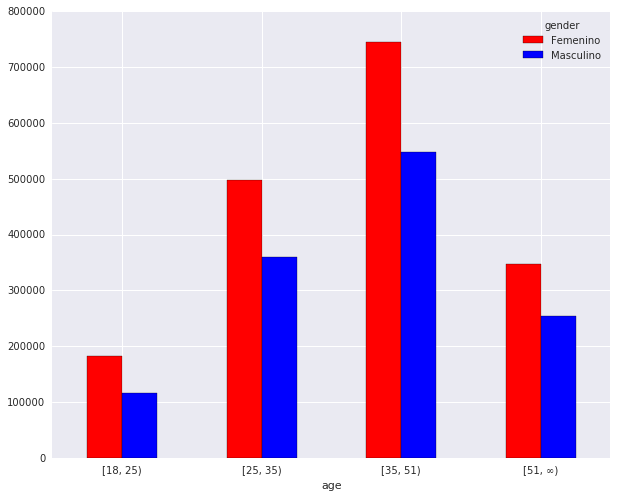
\includegraphics[width=\columnwidth]{Figures/gender_age_bar}
\caption{Cantidad de usuarios en \( G_N \) por genero y edad}
\end{figure}

\begin{figure}
\center
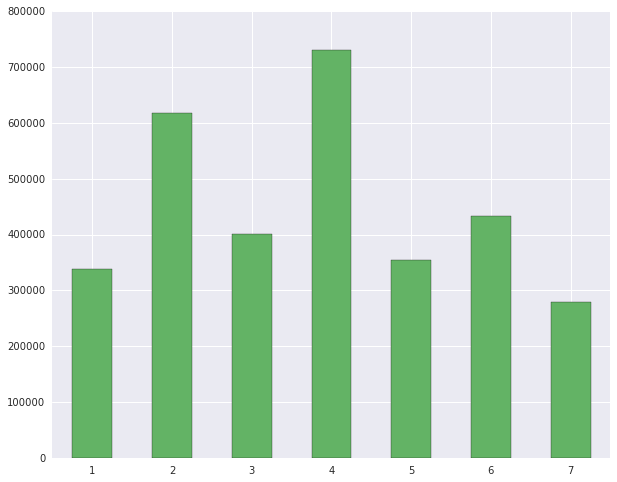
\includegraphics[width=\columnwidth]{Figures/sei_hist}
\caption{Usuarios por nivel socioeconómico}
\end{figure}

\begin{figure}
\center
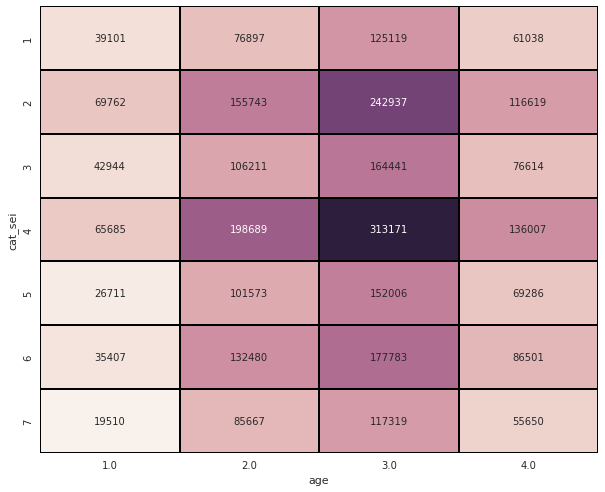
\includegraphics[width=\columnwidth]{Figures/sei_age_heatmap}
\caption{Nivel socioeconomico por genero y edad}
\end{figure}



\bibliographystyle{plain}
% \bibliographystyle{splncs}

\bibliography{bibliography/sna}


\end{document}

